\note{Make this section more about the device and how well it works, less about the actual measurements we got. To talk about the measurements, examine why they match up with literature or not. How is that related to the instrument? Hint: we didn't calibrate shit.}

In order to test the new microspectrometer instrument, we measure the fluorescence spectra of two 

\subsection{ADT TES-F}

\begin{figure}[H]
    \centering
    \begin{subfigure}[b]{0.45\textwidth}
        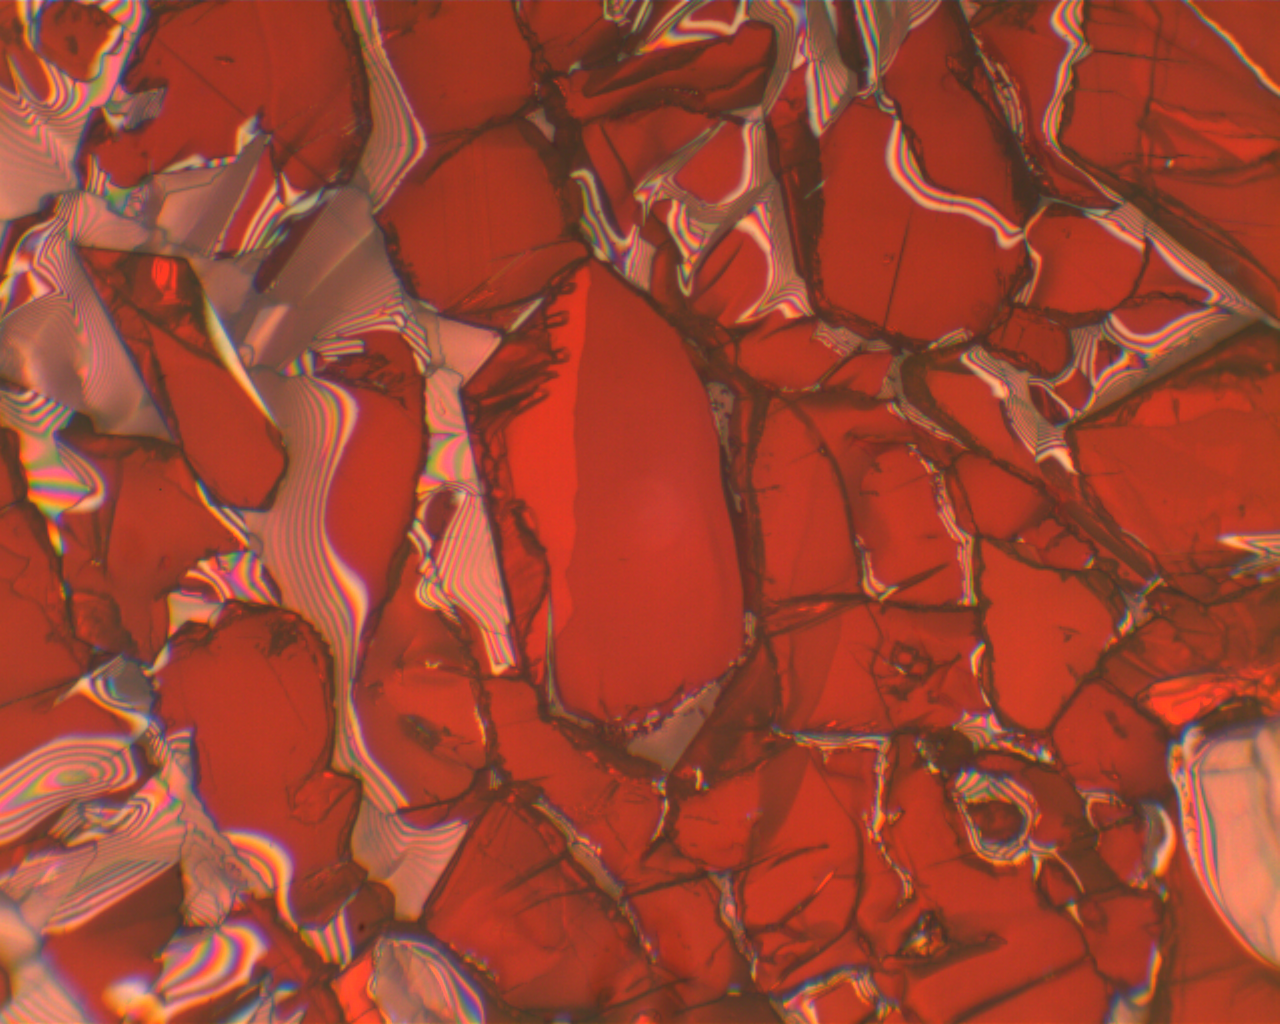
\includegraphics[width=\textwidth]{./img/tesf-white-illum.png}
        % \caption{TESF region of interest under white light.}
        \caption{}
        \label{img:tesf-white}
    \end{subfigure}
    \hfill
    \begin{subfigure}[b]{0.45\textwidth}
        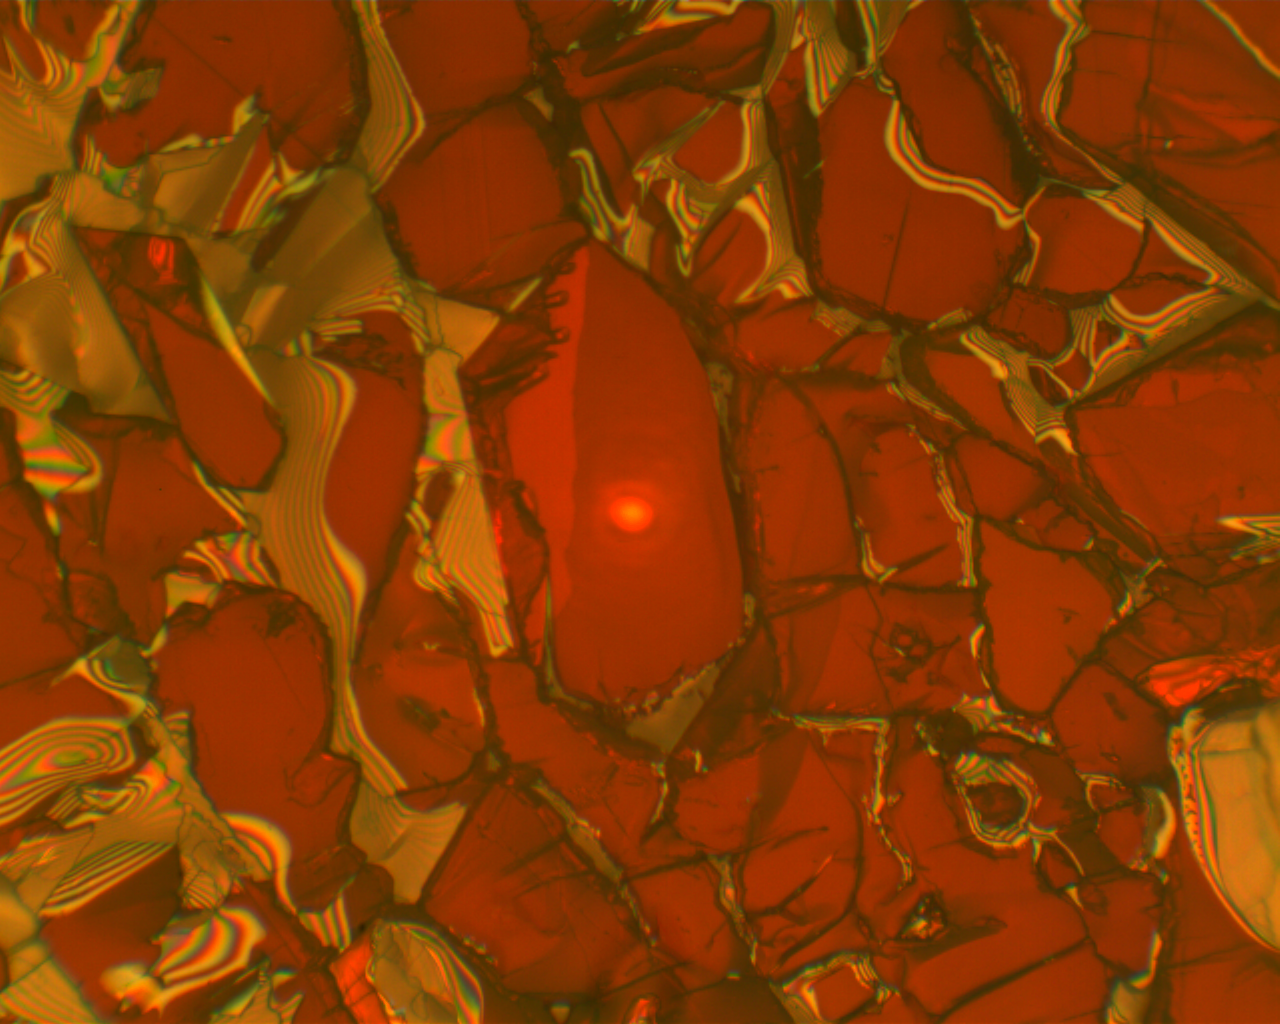
\includegraphics[width=\textwidth]{./img/tesf-laser-illum.png}
        % \caption{TESF region of interest under excitation light.}
        \caption{}
        \label{img:tesf-laser}
    \end{subfigure}
    \caption[Images of ADT TES-F sample.]{Images of ADT TES-F sample under white light (\ref{img:tesf-white}) and under laser excitation light (\ref{img:tesf-laser}). Reflected excitation light was optically filtered out of Figure \ref{img:tesf-laser} using a dichroic mirror and colored glass longpass filter. Photoluminescence spectra of this region are shown in Figure \ref{fig:pl-adt-tesf}.}
    \label{img:tesf}
\end{figure}

\begin{figure}[H]
    \centering
    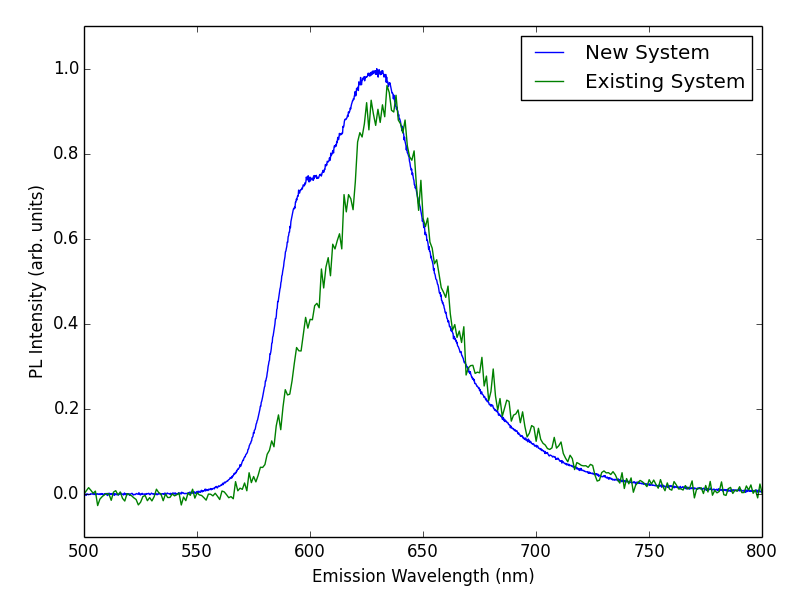
\includegraphics[width=.8\textwidth]{./img/tesf-2.png}%\llap{\raisebox{4cm}{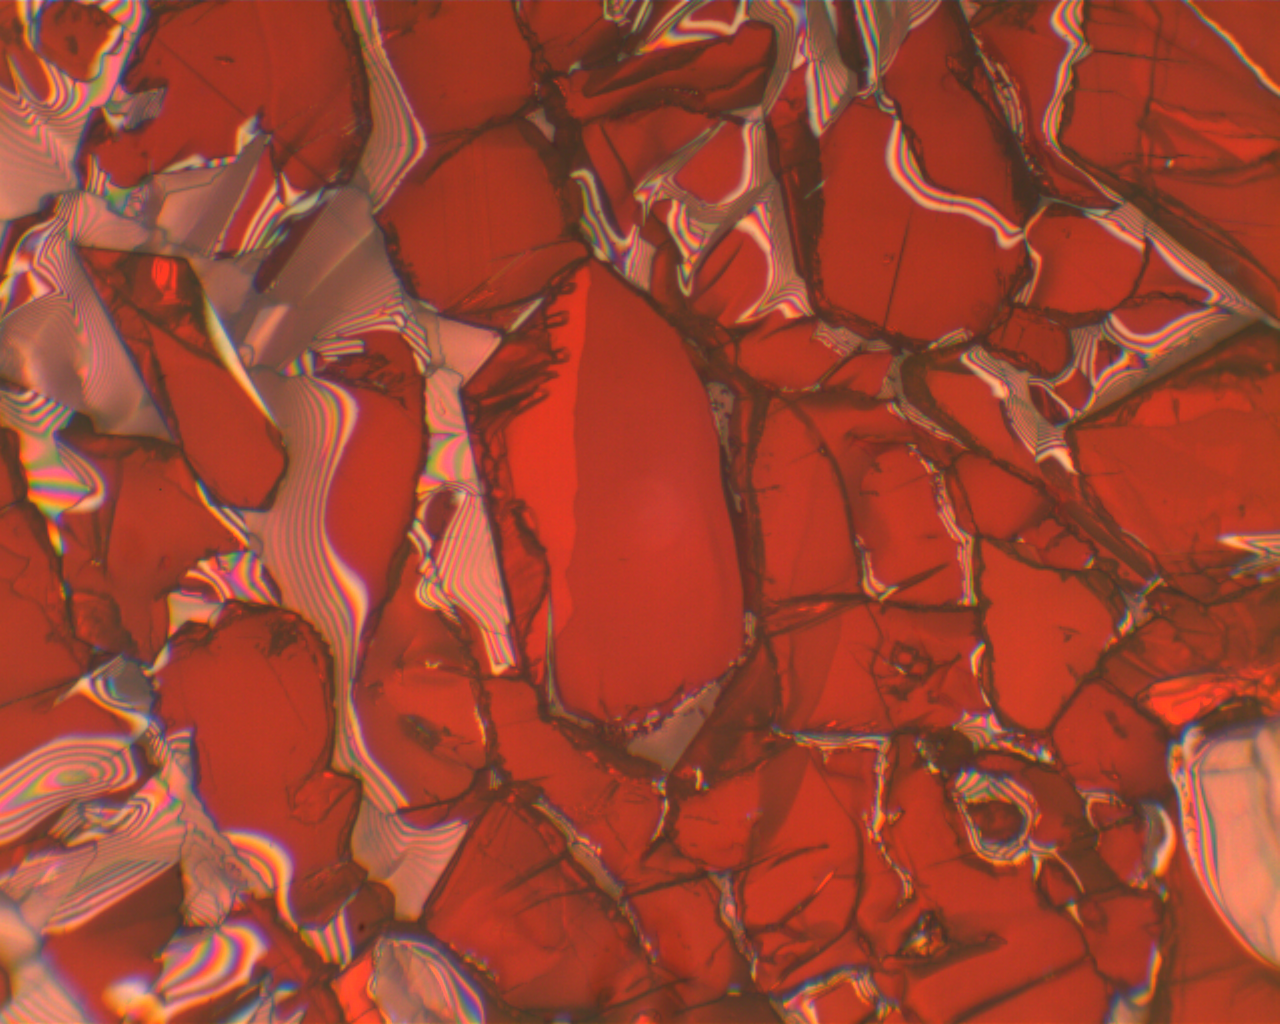
\includegraphics[width=2cm]{img/tesf-white-illum.png}}}
    % 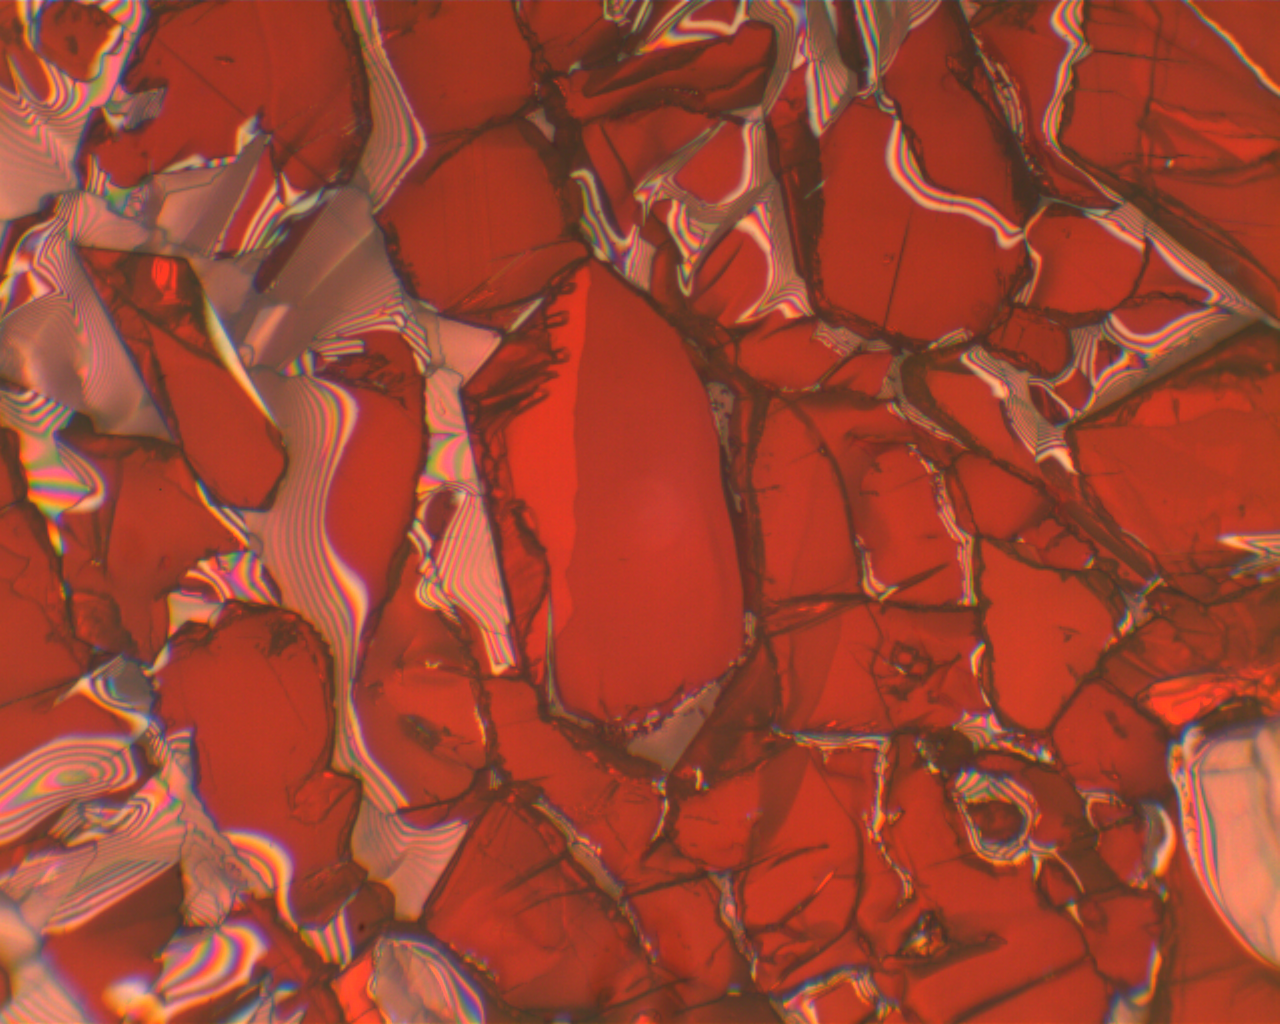
\includegraphics[width=.2\textwidth]{./img/tesf-white-illum.png}
    % 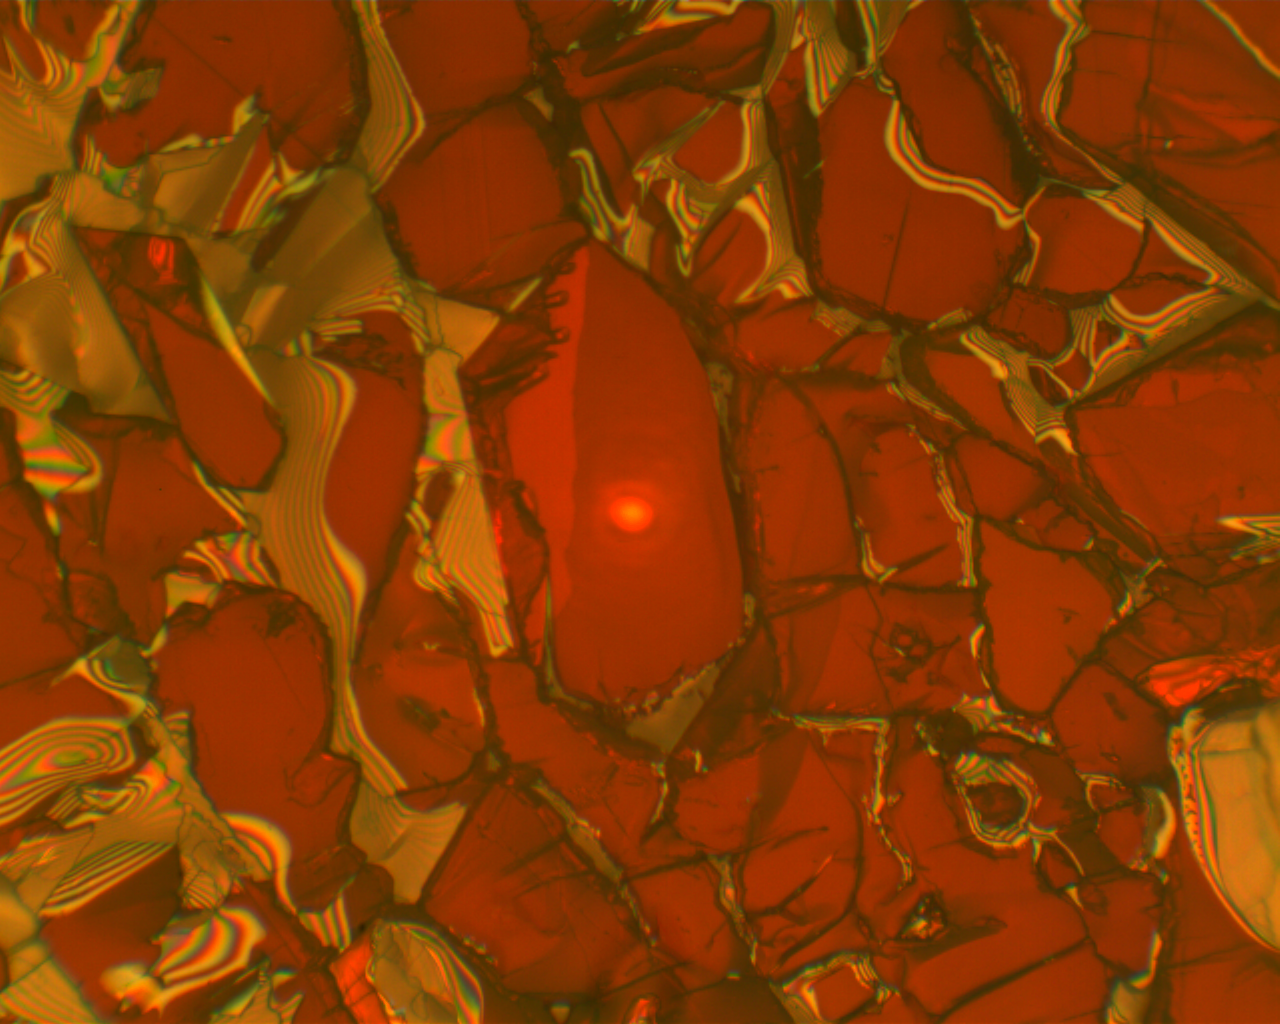
\includegraphics[width=.2\textwidth]{./img/tesf-laser-illum.png}
    \caption[PL emission spectrum of ADT TES-F, excited at 405nm.]{PL emission spectrum of ADT TES-F, excited at 405 nm.
    Wide-field illumination used by the existing system to excite the sample
    yields a noisy spectrum, and does not excite the secondary peak that is 
    shown clearly in the results from the new system. A single crystal, larger than the laser spot, was selected among smaller neighboring crystals for this measurement. %This may be because the
    %wide-field illumination is exciting many adjacent crystals in the sample, 
    %which emit slightly different spectra. The laser illumination in the new 
    %system has the spatial resolution necessary to illuminate single crystals.
    }
    \label{fig:pl-adt-tesf}
\end{figure}

For a drop-cast sample of ADT TES-F on glass, we selected a region of interest which appeared to be a single crystal, with few visually distinguishable defects (Figure \ref{img:tesf}). The crystal was also selected such that its surface area was larger than the area illuminated by the microspectrometer's laser spot. The emission spectra of the region of interest are shown in Figure \ref{fig:pl-adt-tesf}.

Using the fluorimeter instrument, we were able to illuminate and measure the PL spectrum of the same region of interest, plus an indeterminate area of the sample around this region.

Both spectra in Figure \ref{fig:pl-adt-tesf} show a clear peak around 630nm. The spectra measured by the microspectrometer also shows a secondary peak just below 600 nm, which is not evident in the spectrum taken by the fluorimeter. \cite{lam_polarization_2018}\cite{ostroverkhova_organic_2016}\cite{platt_optical_2009}\note{All 3 citations in this paragraph have spectra with peaks similar to mine, but different intensity. This must be because they excited at a different wavelength, but how do I use that?}


\subsection{\ce{CdSe} Quantum Dots}

\begin{figure}[H]
    \centering
    \begin{subfigure}[b]{0.45\textwidth}
        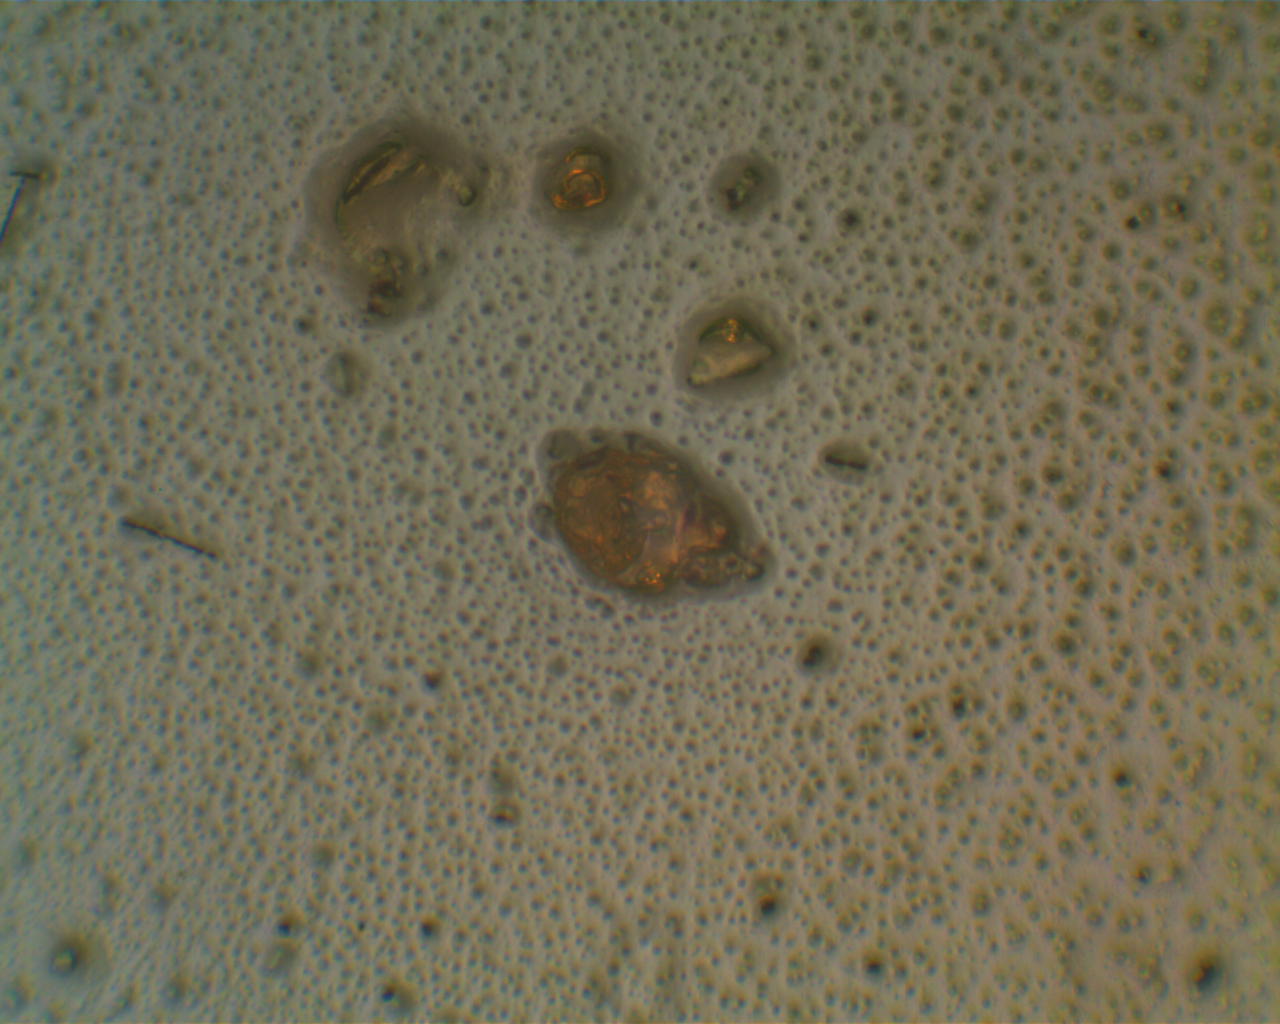
\includegraphics[width=\textwidth]{./img/qd-white-illum.png}
        \caption{}
        \label{img:qd-white}
    \end{subfigure}
    \hfill
    \begin{subfigure}[b]{0.45\textwidth}
        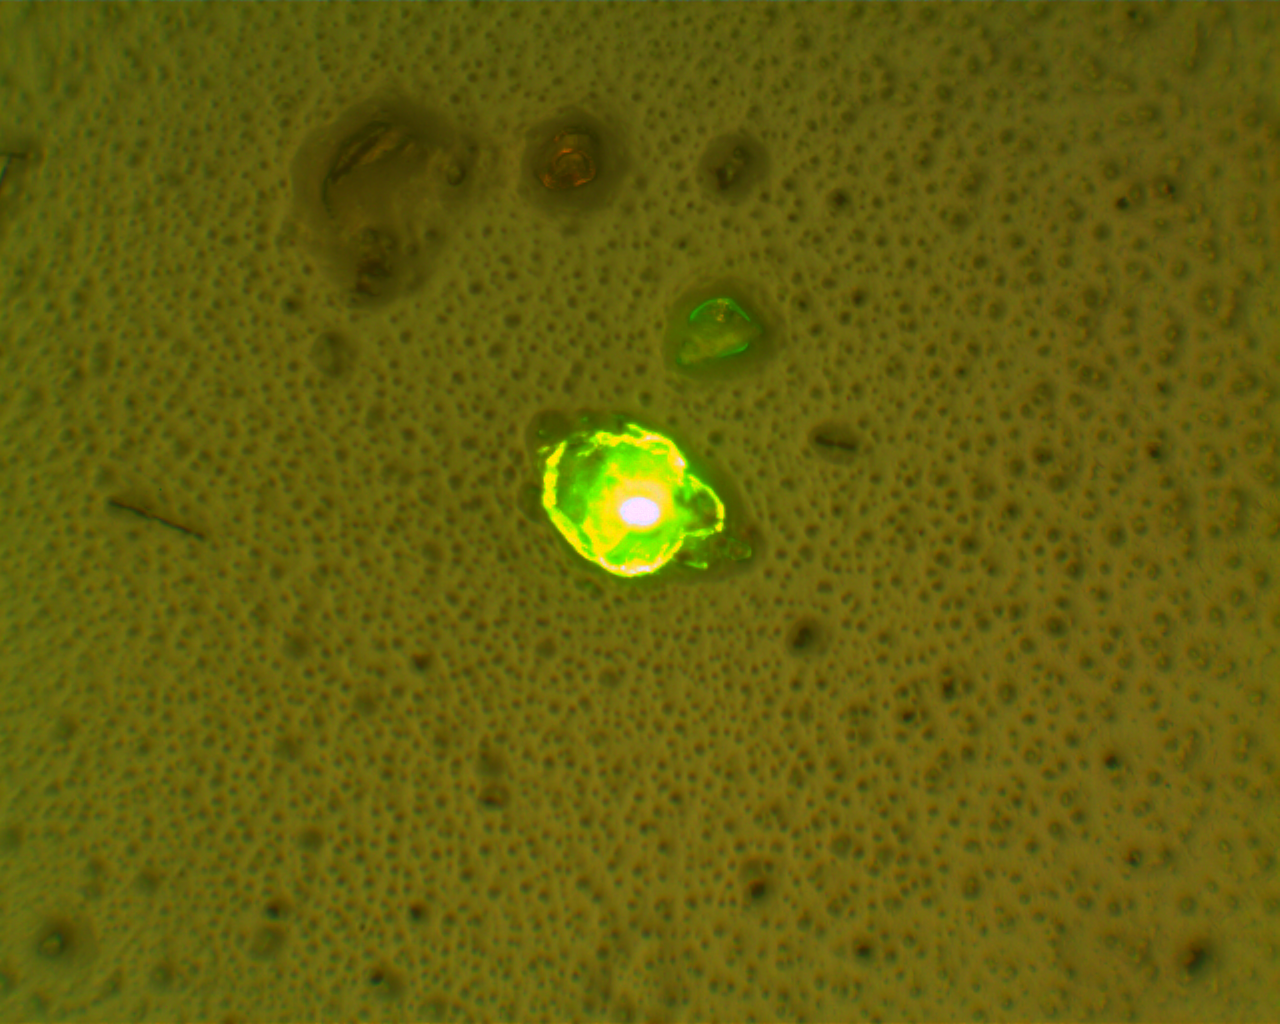
\includegraphics[width=\textwidth]{./img/qd-laser-illum.png}
        \caption{}
        \label{img:qd-laser}
    \end{subfigure}
    \caption[Images of CdSe quantum dot sample.]{Images of CdSe quantum dot sample under white light (\ref{img:qd-white}) and under laser excitation light (\ref{img:qd-laser}). Reflected excitation light was optically filtered out of Figure \ref{img:qd-laser} with a dichroic mirror and colored glass longpass filter. Photoluminescence spectra of this sample are shown in Figure \ref{fig:pl-adt-qd}.}
    \label{img:qd}
\end{figure}

\begin{figure}[H]
    \centering
    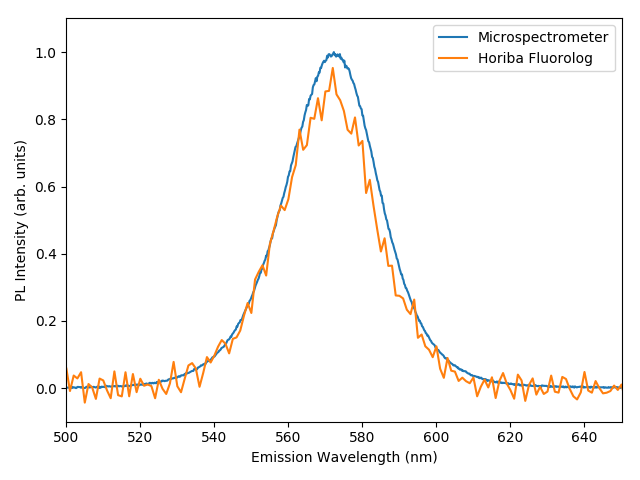
\includegraphics[width=\textwidth]{./img/qd-2.png}
    % 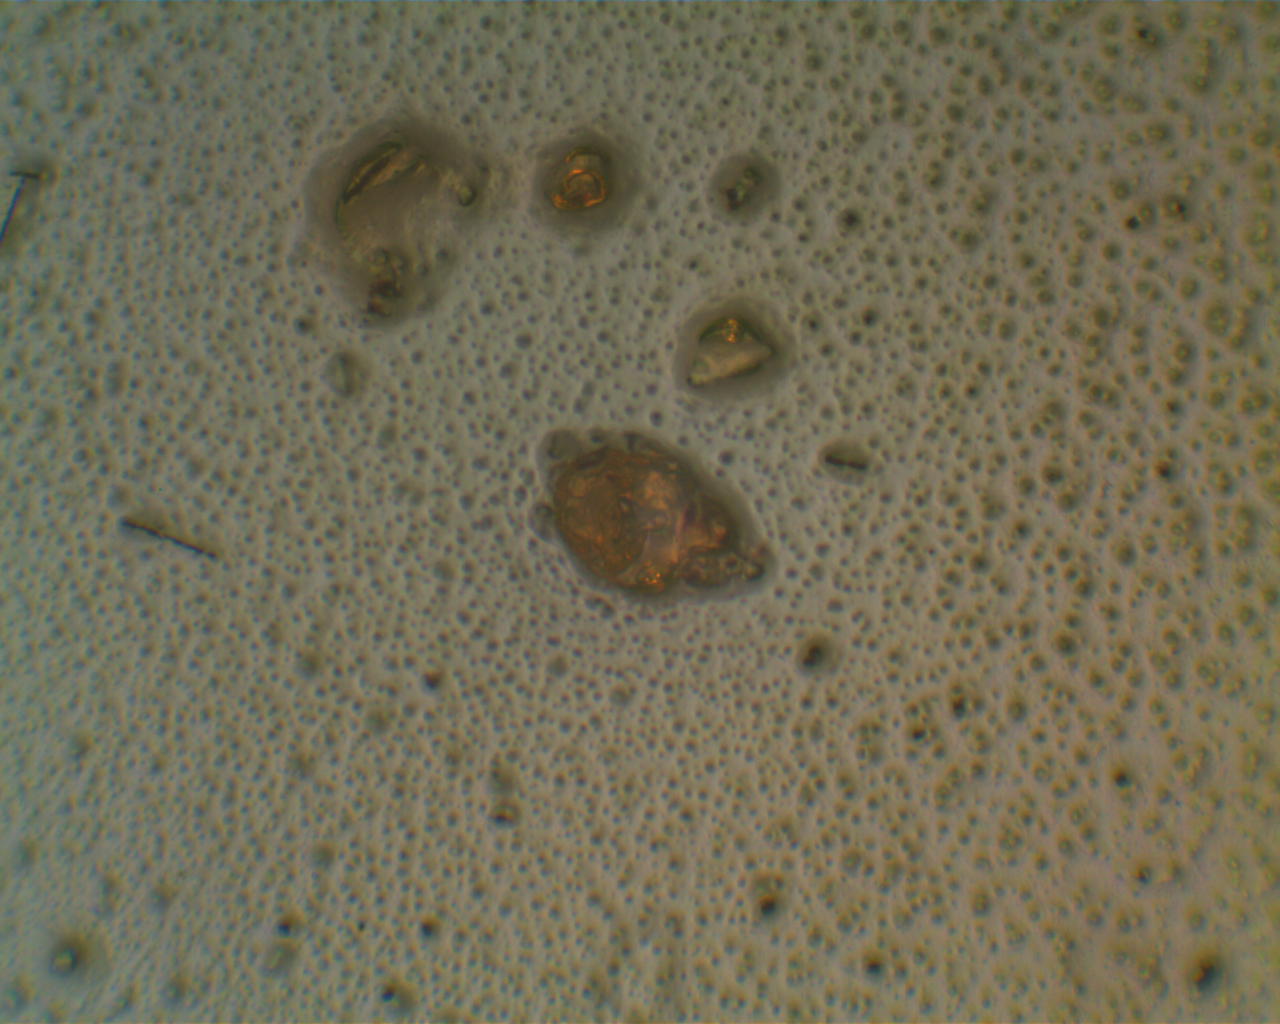
\includegraphics[width=4cm]{./img/qd-white-illum.png}
    % 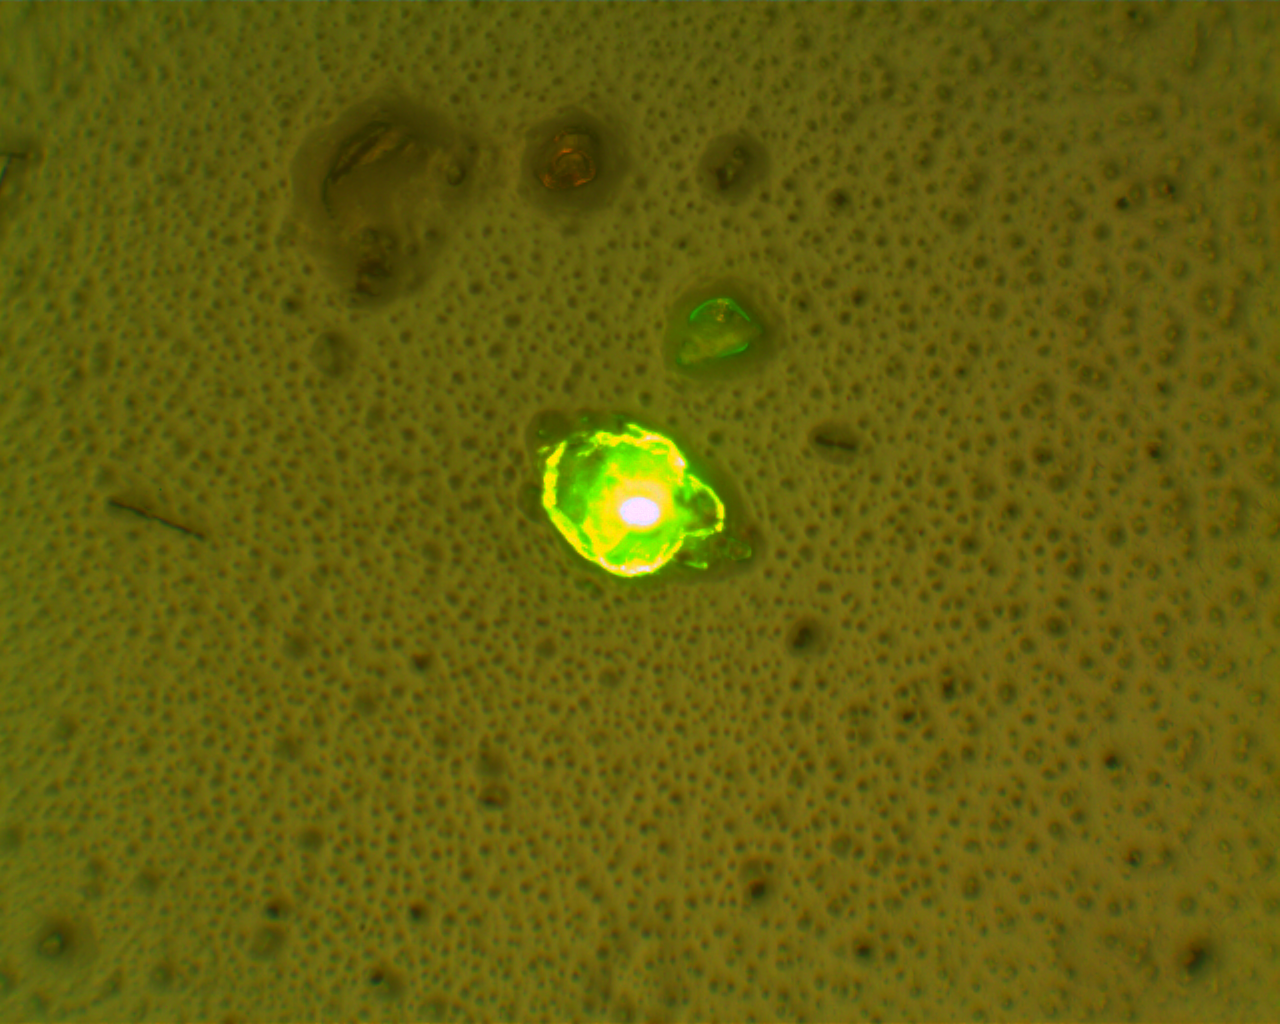
\includegraphics[width=4cm]{./img/qd-laser-illum.png}
    \caption{PL emission spectrum of a cluster of CdSe quantum dots, excited at 405 nm.}
    \label{fig:pl-adt-qd}
\end{figure}

Figure \ref{fig:pl-adt-qd} shows the PL emission of CdSe quantum dots \todo{on what substrate?}. There is one broad, clear peak that aligns well with the same measurement taken on the fluorimeter, between 520 and 620 nm. This peak seems to agree with other studies of CdSe quantum structures.\cite{empedocles_photoluminescence_1996}

Unlike the same measurement taken on ADT, this measurement was taken in a region of interest which is sparsely populated with quantum dots, with one target grouping illuminated by the laser.

\todo{What else do I write about here? Need to find more resources on analysis of PL, i.e. what information we get about the material. This will also be useful for Background section.}
